\section{Question 3-Natural Response}
It was proposed to study and determine the natural response of the circuit over time, in node 6. The natural response of the circuit is what the circuit does including the initial conditions (initial voltage of the capacitor) but with the imput supressed. 

\subsection{Theoretical Analysis}




\subsection{Simulation Analysis}
In this section, a transient analysis was made in order to evaluate the natural response of the circuit, which means, the variation over time. The description of the circuit included the initial values of v(6) and v(8), calculated in question 1. As the ngspice and octave results matched, as observed in \ref{subsection:2.3}, the theorectical values were imported from a .cir file created by octave.
The time interval considered was [0,20]ms.
\begin{figure}[ht] \centering
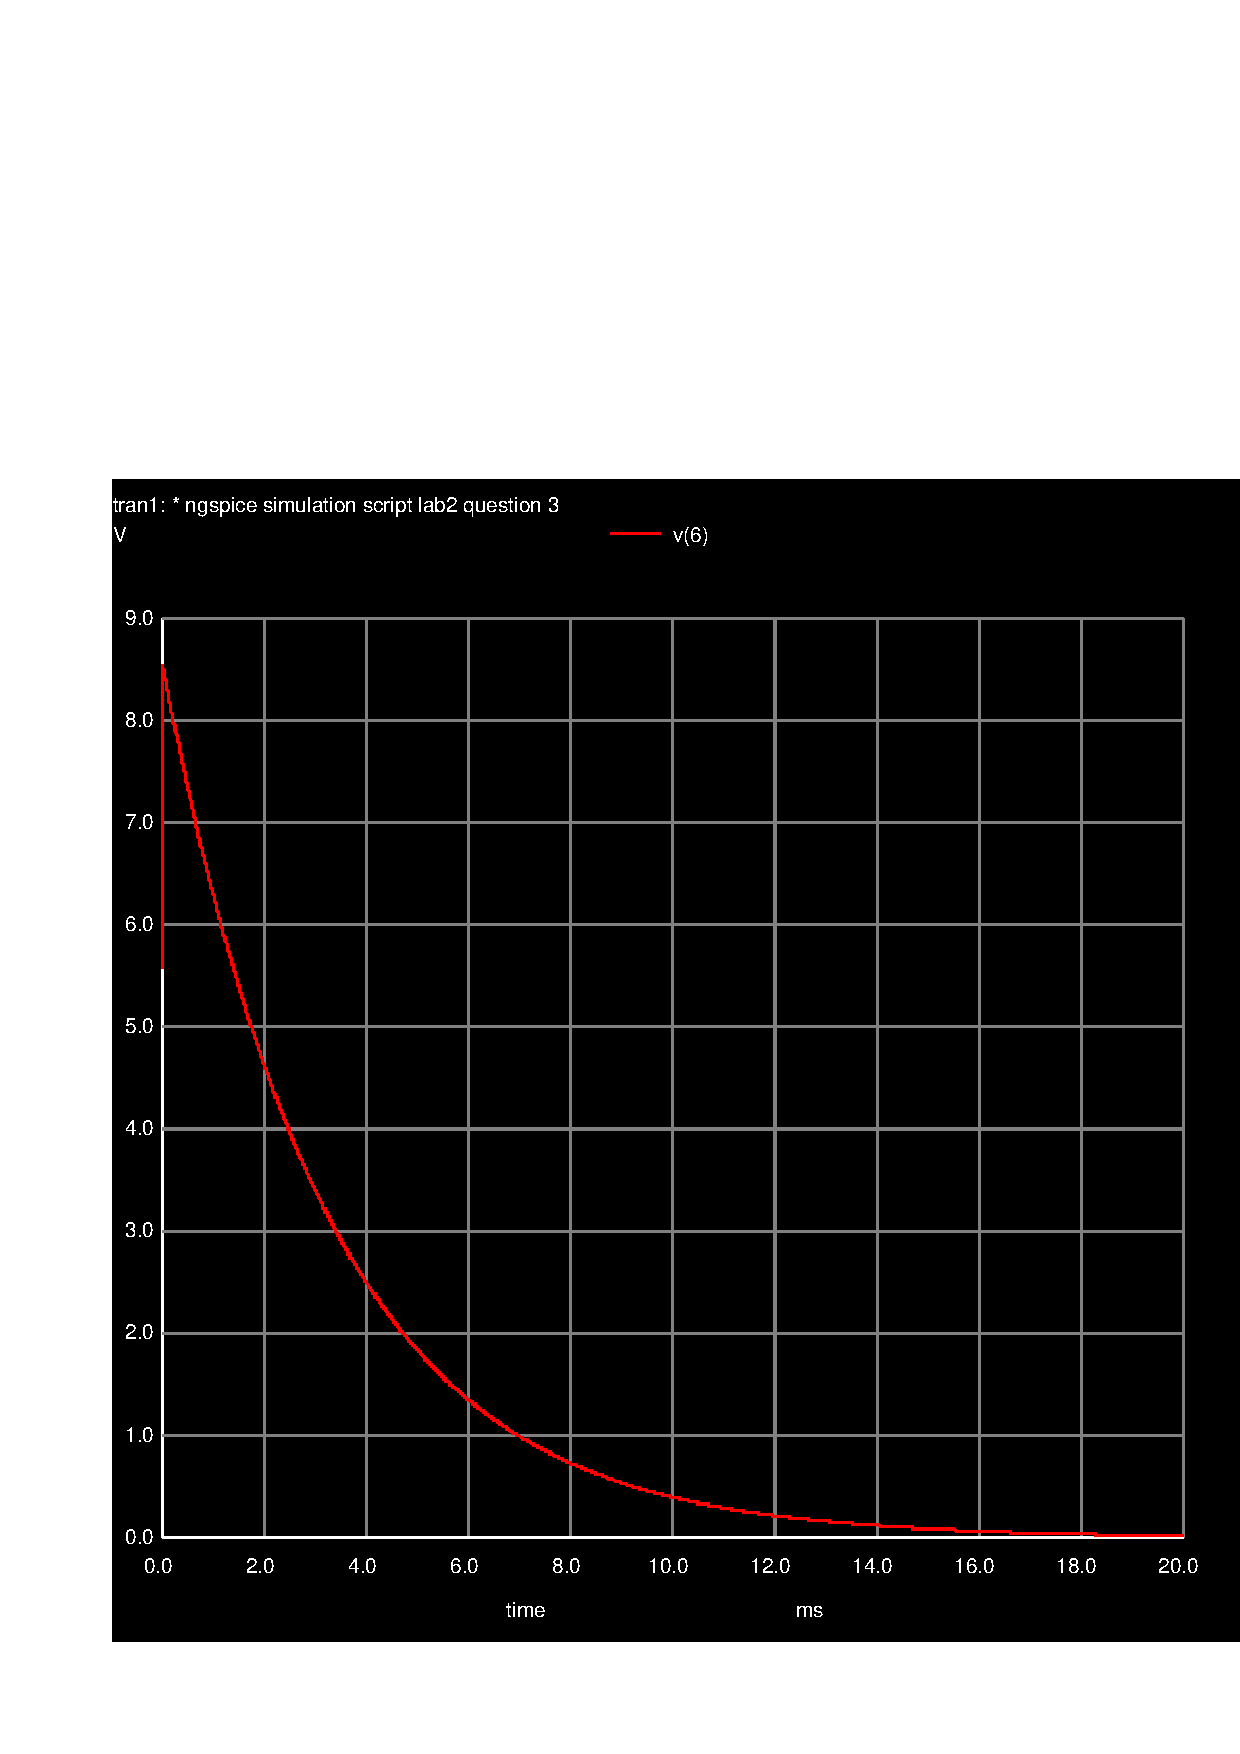
\includegraphics[width=0.9\linewidth]{sim3.pdf}
\caption{Circuit analysed.}
\label{fig:sim3}
\end{figure}
